\chapter{Конструкторский раздел}
\label{cha:design}

\section{Модель объектно-ориентированной системы}

Для поиска шаблонов проектирования нужно привести программу и шаблон к одному представлению.
За основу можно взять UML-диаграммы классов.
В них не хватает явных определений некоторых необходимых связей, например, вызовов методов.
Такие связи, обычно, указываются в комментариях к элементам диаграммы.

В UML-диаграммах довольно много элементов, при описании шаблонов проектирования используется только часть.
Убрав все лишнее и добавив нужные связи получим структуру модели представленную на рисунке~\ref{fig:model}.

\begin{figure}[!ht]
\centering
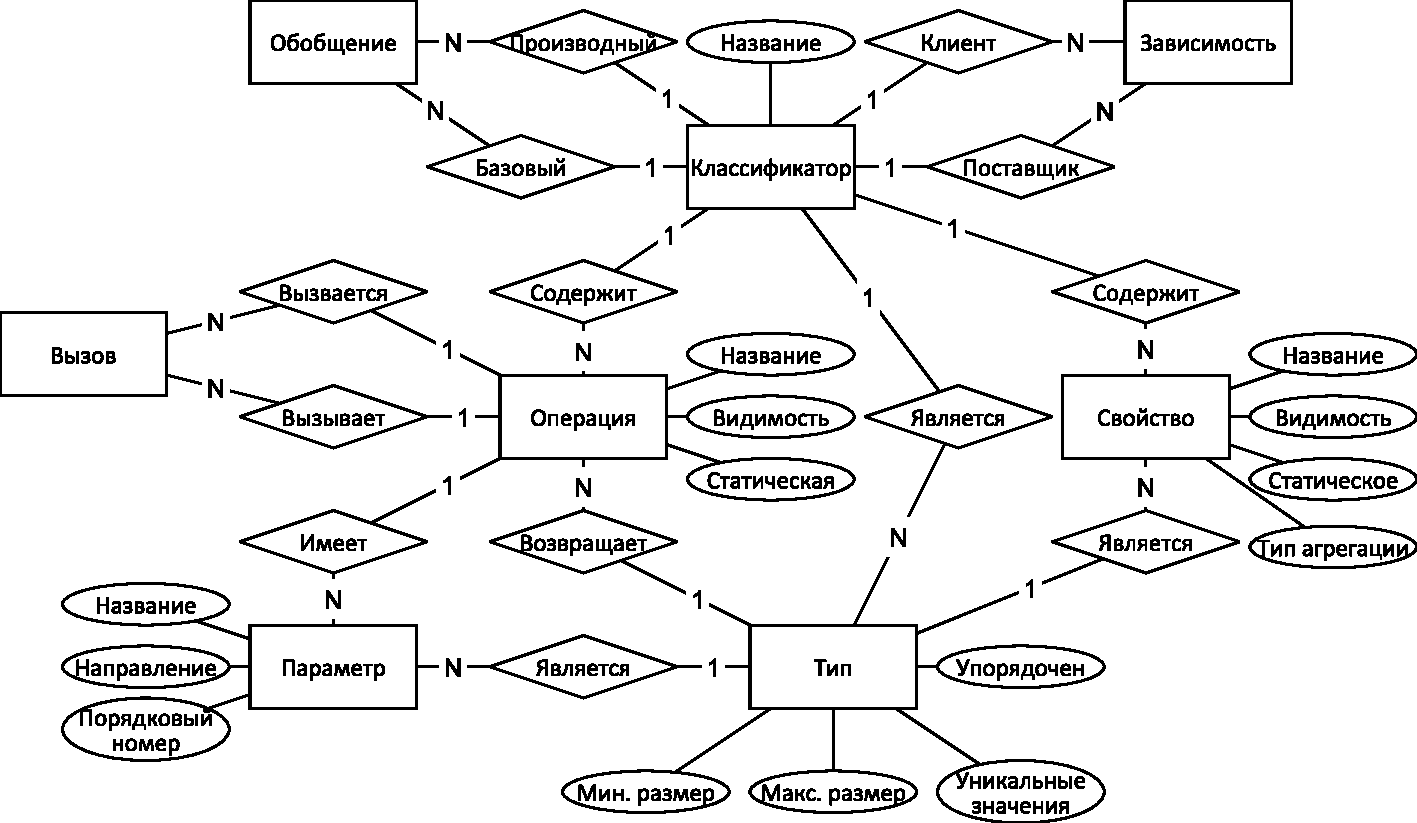
\includegraphics[width=\textwidth]{inc/model.pdf}
\caption{Структура модели объектно-ориентированной системы}
\label{fig:model}
\end{figure}

\section{Граф со множеством типов дуг}

Поиск шаблонов проектирования можно выполнять, выполняя поиск изоморфного подграфа в графе.
Типы вершин можно не различать, если считать, что в графе не может существовать двух эквивалентных вершин.
Описанная модель сожержит множество типов связей.
Может существовать несколько типов связей между вершинами.
Введем множество типов дуг, обозначив каждый тип меткой.
Структура графа представлена на рисунке~\ref{fig:graph}.

\begin{figure}[!ht]
\centering
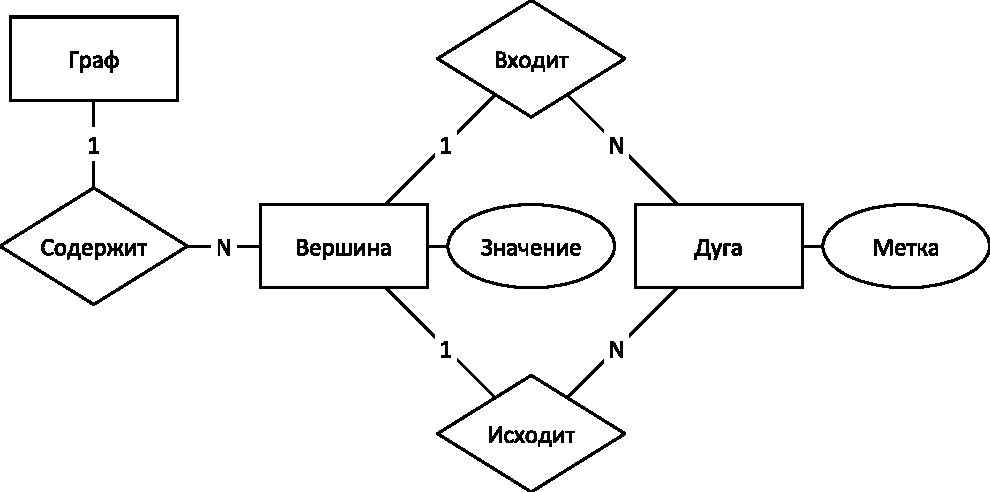
\includegraphics[width=0.8\textwidth]{inc/graph.pdf}
\caption{Структура графа с множеством типов дуг}
\label{fig:graph}
\end{figure}

\section{Алгоритм поска изоморфных подграфов с множеством типов дуг}

Рассмотренный ранее алгоритм Ульмана для поиска изоморфных подграфов,
не подходит для ориентированных графов с множеством типов дуг.
Нужен новый алгоритм.
За основу можно взять метод поиска в глубину, условие эквивалентности вершин
и процедуру <<отсеивания>> лишних эквивалентностей.

Общая идея алгоритма заключается в том,
что нужно для кажой вершины целевого графа найти эквивалентные вершины в шаблоне,
а затем переходя по дугам, без учета направлений,
по одной вершине добавлять к возможному изоморфному подграфу.
На каждом шаге нужно проверять корректность решения.
Таким образом, у алгоритма есть состояние на каждом шаге --- конфигурация.
Каждая конфигурация может породить множество конфигураций.
Конфигурация является конечной, если больше не осталось вершин шаблона,
которым можно сопоставить вершину целевого графа.
Результат алгоритма --- все возможные варианты множеств пар изоморфных вершин,
в каждом множестве представлены все вершины шаблона.

Для начала введем понятие эквивалентности вершин.
Обозначим некоторые величины:
\begin{itemize}
\item $target$ --- целевой граф;
\item $pattern$ --- граф шаблона;
\item $L_G$ --- множество меток дуг графа $G$;
\item $incoming^{l}_G$ --- множество входящих дуг с меткой $l$ вершины графа $G$;
\item $outgoing^{l}_G$ --- множество исходящих дуг с меткой $l$ вершины графа $G$;
\item $object_G$ --- значение вершины графа $G$;
\end{itemize}

\textbf{Определение}. $isEquivalent: Object \times Object \to \{ 0, 1 \}$ ---
функция эквивалентности значений вершин.
%
$$object_{G_1} \cong object_{G_2} \iff isEquivalent(object_{G_1}, object_{G_2})$$

\textbf{Определение}. Вершины эквивалентны ($target \cong pattern $), если:
\begin{enumerate}
\item $( \forall l \in L_{pattern} ) ( |incoming^{l}_{target}| \ge |incoming^{l}_{pattern}| )$;
\item $( \forall l \in L_{pattern} ) ( |outgoing^{l}_{target}| \ge |outgoing^{l}_{pattern}| )$;
\item $object_{target} \cong object_{pattern}$.
\end{enumerate}

Введем обозначение графа.

\textbf{Определение}. $G = ( V, L, E )$ --- граф с множеством типов дуг, где
\begin{itemize}
\item $V = \{ v \}$ --- множество вершин;
\item $L = \{ l \}$ --- множество меток дуг;
\item $E = \{ e = (u, v, l) :  u, v \in V \land l \in L \}$ --- множество дуг.
\end{itemize}

Последовательность конфигураций от начальной до конечной приводит к получению
очередного множества пар эквивалентных вершин, и имеет определенную структуру.

\textbf{Определение}. $C = ( selected, current, checked )$ --- конфирурация
алгоритма поиска подграфов с множеством типов дуг, где
\begin{itemize}
\item $selected = \{ e^n = ( v^n_{target}, v^n_{pattern} ) \}_{n=1}^N$ ---
последовательность пар вершин целевого графа и шаблона, которые прошли проверку
или требуют проверки;
\item $current \in \N$ --- номер элемента из $selected$;
\item $checked = \{ ( v_{target}, v_{pattern} ) \}$ --- множество проверенных
пар вершин, гарантируется, что построенные из вершин этого множества графы
изоморфны.
\end{itemize}

\textbf{Определение}. Конфигурация является начальной, если:
\begin{enumerate}
\item $selected = \{ e^n \}_{n=1}^N, N \ge 1$;
\item $current = 1$;
\item $checked = \{ e^1 \}$.
\end{enumerate}

\textbf{Определение}. Конфигурация является конечной, если $current > |selected|$.

Определим функции, использующиеся в алгоритме.

\textbf{Определение}. $\textrm{NEIGHBORS} : V \to 2^V$ --- множество соседей вершины графа:
%
$$\textrm{NEIGHBORS}(v_G) = \{ u : (u \ne v_G) \land ( ( \exists (u, v_G, l^i_G) \in E_G ) | ( \exists (v_G, v, l^j_G) \in E_G ) ) \}$$

\textbf{Определение}. $\textrm{CHAINS} : 2^V \times 2^V \to 2^{Chain}$ --- множество последовательностей пар вершин, изоморфизм которых нужно поверить:
%
$$Chain = \{ ( v^n_t, v^n_p ) : ( v^n_t \cong v^n_p ) \land ( ( \forall i, j ) ( v^i_t \ne v^j_t \land v^i_p \ne v^j_p ) ) \}_{n = 1}^N$$
%
$$\textrm{CHAINS}(V_t, V_p) = \{ Chain = \{ ( v^n_t, v^n_p ) \}_{n = 1}^N : ( v^n_t \in V_t ) \land ( v^n_p \in V_p ) \}$$

\textbf{Определение}. $\textrm{CHECKED\_TARGETS} : 2^C \to 2^V$ --- вершины целевого графа из множества проверенных пар конфигурации:
%
$$\textrm{CHECKED\_TARGETS}(C) = \{ v_{target} : ( v_{target}, v_{pattern} ) \in checked_C \}$$

\textbf{Определение}. $\textrm{CHECKED\_PATTERNS} : 2^C \to 2^V$ --- вершины шаблона из множества проверенных пар конфигурации:
%
$$\textrm{CHECKED\_PATTERNS}(C) = \{ v_{pattern} : ( v_{target}, v_{pattern} ) \in checked_C \}$$

\textbf{Определение}. $\textrm{IS\_VALID} : 2^C \to \{ 0, 1 \}$ --- может ли конфигурация привести к изоморфизму:
%
$$\textrm{IS\_VALID}(C) = T_{outgoing} \subseteq P_{outgoing} \land T_{incoming} \subseteq P_{incoming} $$
%
\begin{itemize}
\item $(target, pattern) = selected^{current}_C$
\item $(V_{target}, E_{target}) = G_{target}, target \in V_{target}$ --- граф, в котором находится вершина $target$;
\item $(V_{pattern}, E_{pattern}) = G_{pattern}, pattern \in V_{pattern}$ --- граф, в котором находится вершина $pattern$;
\item $T_{outgoing} = \{ c : ( target, v, c ) \in E_{target} \land v \in \textrm{CHECKED\_TARGETS}(C) \} $;
\item $T_{incoming} = \{ c : ( v, target, c ) \in E_{target} \land v \in \textrm{CHECKED\_TARGETS}(C) \} $;
\item $P_{outgoing} = \{ c : ( pattern, v, c ) \in E_{pattern} \land v \in \textrm{CHECKED\_PATTERNS}(C) \} $;
\item $P_{incoming} = \{ c : ( v, pattern, c ) \in E_{pattern} \land v \in \textrm{CHECKED\_PATTERNS}(C) \} $.
\end{itemize}

\textbf{Определение}. ADD --- процедура, добавляющаяя конфигурации в
коллекцию конфигураций. Реализация зависит от типа коллекции.

\textbf{Определение}. TAKE --- извлекает из коллекции конфигураций
очередную конфигурацию. Реализация зависит от типа коллекции.

Коллекция конфигураций может быть стеком, очередью или другой структурой данных.
Функции ADD и TAKE соответствено могут добавлять в конец стека или извлекать,
добавлять в конец очереди, извлекать с начала очереди.
Можно использовать асинхронные структуры данных и ленивые вычисления,
что может быть более эффективно, если нужно получить первые $N$ изоморфизмов.
Также можно использовать приоритеты, например, мощность множества $checked$.

\textbf{Определение}. Алгоритм генерации начальных конфигураций:

\textbf{Входные данные}:
\begin{itemize}
\item $V_t$ --- множество вершин целевого графа;
\item $V_p$ --- множество вершин шаблона.
\end{itemize}

\textbf{Результат}: $\{ C \}$ --- множество начальных конфигураций.

\begin{algorithmic}
\Function{initial\_configurations}{$V_t$, $V_p$}
    \State $C \gets \varnothing$
    \State $p \gets v : |$\Call{neighbors}{$v$}$| = \min\limits_{w \in V_p} \{ |$\Call{neighbors}{$w$}$| \}$
    \ForAll{ $( v_t, p ) : ( v_t \cong p ) \land ( v_t \in V_t ) $ }
        \ForAll{ $chain \in$ \Call{chains}{ \Call{neighbors}{$v_t$}, \Call{neighbors}{$v_p$} } }
            \State $C \gets C \ \cup \{$ \Call{make\_configuration}{$v_t$, $v_p$, $chain$} $\}$
        \EndFor
    \EndFor
    \State \Return $C$
\EndFunction
\end{algorithmic}

\textbf{Определение}. Алгоритм <<продвижения>> конфигурации.

\textbf{Входные данные}: $C$ --- не конечная конфигурация.

\textbf{Результат}: $C$ --- конечная конфигурация или конфигурация с новым
элементом в множестве $checked$.

\begin{algorithmic}
\Function{advance}{$C$}
    \State $(selected, current, checked) \gets C$
    \State $checked\_t \gets$ \Call{checked\_targets}{$C$}
    \State $checked\_p \gets$ \Call{checked\_patterns}{$C$}
    \While{$true$}
        \State $current \gets current + 1$
        \State $C_{next} \gets (selected, current, checked)$
        \If{$current > |selected|$}
            \State \Return $C_{next}$
        \EndIf
        \State $(target, pattern) \gets selected^{current}$
        \If{$target \not\in checked\_t \land pattern \not\in checked\_p \land$ \Call{is\_valid}{$C_{next}$}}
            \State \Return $(selected, current, checked \cup \{ selected^{current} \})$
        \EndIf
    \EndWhile
\EndFunction
\end{algorithmic}

\textbf{Определение}. Агоритм построения производных конфигураций.

\textbf{Входные данные}: $C$ --- неконечная конфигурация.

\textbf{Результат}: $\{ C \}$ --- множество производных конфигураций.

\begin{algorithmic}
\Function{derived\_configurations}{$C$}
\State $result \gets \varnothing$
\State $(selected, current, checked) \gets C$
\State $(v_t, v_p) \gets selected^{current}$
\ForAll{ $chain \in$ \Call{chains}{ \Call{neighbors}{$v_t$}, \Call{neighbors}{$v_p$} } }
    \State $addition \gets chain \setminus selected$
    \If{ $addition \ne \varnothing$ }
        \State $result \gets result \cup \{ (selected \cdot addition, current, checked) \}$
    \EndIf
\EndFor
\If{ $result = \varnothing$ }
    \State $result \gets \{ C \}$
\EndIf
\State \Return $result$
\EndFunction
\end{algorithmic}

\textbf{Определение}. Агоритм поиска изоморфного подграфа в графе с одной
компонентой связности.

\textbf{Входные данные}:
\begin{itemize}
\item $G_{target}$ --- целевой граф;
\item $G_{pattern}$ --- граф шаблона.
\end{itemize}

\textbf{Результат}: $\{ \{ ( v_{target}, v_{pattern} ) \} \}$ --- множество
изоморфизмов.

\begin{algorithmic}
\Function{match\_one}{$G_{target}$, $G_{pattern}$}
    \State $isomorphisms \gets \varnothing$
    \State $Configurations \gets$ \Call{initial\_configurations}{$G_{target}$, $G_{pattern}$}
    \While{$Configurations \ne \varnothing$}
        \State $Configurations, C \gets$ \Call{take}{$Configurations$}
        \State $C \gets$ \Call{advance}{C}
        \If{$C$ --- конечная конфигурация}
            \If{\Call{checked\_patterns}{$C$} $= V_{pattern}$}
                \State $isomorphisms \gets isomorphisms \cup \{ checked_C$ \}
            \EndIf
        \Else
            \State $Configurations \gets$ \Call{add}{$Configurations$, \Call{derived\_configurations}{$C$} }
        \EndIf
    \EndWhile
    \State \Return $isomorphisms$
\EndFunction
\end{algorithmic}

Конфигурации не связаны, поэтому их проверка может выполняться параллельно.
В этом алгоритме тело цикла \textbf{while} может выполняться параллельно,
для этого нужно обеспечить синхронизацию коллекции $Configurations$.

В общем случае графы состоят из нескольких компонент связности.
Чтобы выполнить поиск таких графов, можно выполнить поиск для отдельных компонент,
а затем объеденить результаты.

В этой работе будем считать, что шаблон должен содержать только одну
компоненту связности.

\textbf{Определение}. $\textrm{COMPONENTS} : G \to 2^G$ --- множество компонент
связности графа:

$\textrm{COMPONENTS}(G) = \{ (V, L, E) : V \subseteq V_G \land L \subseteq L_G \land E \subseteq E_G \land (\forall u, v \in V)(\exists \{ w_1 = u, \dots, w_n, \dots, w_N = v : (\forall w_n, n=\overline{2,N})(w_{n-1} \in \textrm{NEIGHBORS}(w_n)) \})$

\textbf{Определение}. Агоритм поиска изоморфного подграфа в графе с множеством
компонент связности.

\textbf{Входные данные}:
\begin{itemize}
\item $G_{target}$ --- целевой граф;
\item $G_{pattern}$ --- граф шаблона.
\end{itemize}

\textbf{Результат}: $\{ \{ ( v_{target}, v_{pattern} ) \} \}$ --- множество
изоморфизмов.

\begin{algorithmic}
\Function{match\_graph}{$G_{target}$, $G_{pattern}$}
    \State $isomorphisms \gets \varnothing$
    \ForAll{ $component \in$ \Call{components}{$G_{target}$}}
        \State $isomorphisms \gets isomorphisms \cup$ \Call{match\_graph}{component, $G_{pattern}$}
    \EndFor
    \State \Return $isomorphisms$
\EndFunction
\end{algorithmic}

Описанный алгоритм не имеет доказательстка корректности.
Вместо этого его результат проверяется на корректность.
Проверяются случаи, когда найденный изоморфизм ложный.
Основная идея состоит в том, что нужно проверить,
действительно ли вершины целевого графа соответствуют вершинам шабона.

Нужно проверить, что:
\begin{enumerate}
\item связи вершины шаблона сооветствуют связям цели;
\item вершины, связанные с вершиной шаблона, изоморфны вершинам цели.
\end{enumerate}

\textbf{Определение}. Условие корректности изоморфизма $I$ подграфа графа
$G_t = (V_t, L_t, E_t)$ и графа $G_p = (V_p, L_p, E_p)$, где $I = \{ (t, p) : t \in V_t \land p \in V_p \}$:
%
$$(\forall (t, p) \in I)$$
$$( (\forall (p, p_x, l) \in E_p)(\exists (t, t_y, l) \in E_t: (t_y, p_x) \in I) \land (\forall (p_a, p, l) \in E_p)(\exists (t_b, t, l) \in E_t: (t_b, p_a) \in I) )$$

\section{Граф модели объектно-ориентированной программы}

На основе модели нужно построить граф, где разные типы связей будут разными типами дуг.
Введеем обозначения:
\begin{itemize}
\item $V_{Classifier} = \{ v_{Classifier} \}$ --- множество вершин, которые являются объектами класса \textbf{Classifier};
\item $V_{Type} = \{ v_{Type} \}$ --- множество вершин, которые являются объектами класса \textbf{Type};
\item $V_{Property} = \{ v_{Property} \}$ --- множество вершин, которые являются объектами класса \textbf{Property};
\item $V_{Operation} = \{ v_{Operation} \}$ --- множество вершин, которые являются объектами класса \textbf{Operation};
\item $V_{Parameter} = \{ v_{Parameter} \}$ --- множество вершин, которые являются объектами класса \textbf{Parameter}.
\end{itemize}

\textbf{Определение}. $Generalization$ --- метка дуги для связи <<обобщение>>
%
$$e_{Generalization} = (v_{derived}, v_{general}, Generalization) : v_{derived}, v_{general} \in V_{Classifier}$$

\begin{itemize}
\item $v_{general}$ --- базовый класс;
\item $v_{derived}$ --- производный класс от $v_{general}$ класс.
\end{itemize}

\textbf{Определение}. $Dependency$ --- метка дуги для определения зависимости
между классами
%
$$e_{Dependency} = (v_{client}, v_{supplier}, Dependency) : v_{client}, v_{supplier} \in V_{Classifier}$$

\begin{itemize}
\item $v_{supplier}$ --- используемый класс;
\item $v_{client}$ --- использующий $v_{supplier}$ класс.
\end{itemize}

\textbf{Определение}. $HasProperty$ --- метка дуги для связи классов и их свойств
%
$$e_{HasProperty} = (v_{Classifier}, v_{Property}, HasProperty)$$

\textbf{Определение}. $HasOperation$ --- метка дуги для связи классов и их операций
%
$$e_{HasOperation} = (v_{Classifier}, v_{Operation}, HasOperation)$$

\textbf{Определение}. $PropertyType$ --- метка дуги для связи свойства и его типа
%
$$e_{PropertyType} = (v_{Property}, v_{Type}, PropertyType)$$

\textbf{Определение}. $OperationResult$ --- метка дуги для связи операции и возвращаемого типа
%
$$e_{OperationResult} = (v_{Operation}, v_{Type}, OperationResult)$$

\textbf{Определение}. $TypeClassifier$ --- метка дуги для связи типа и его класса
%
$$e_{TypeClassifier} = (v_{Type}, v_{Classifier}, TypeClassifier)$$

\textbf{Определение}. $Invocation$ --- метка дуги для связи вызываемой и вызввающей операции
%
$$e_{Invocation} = (v_{invoker}, v_{invoked}, Invocation)$$
%
\begin{itemize}
\item $v_{invoked}$ --- вызываемая операция;
\item $v_{invoker}$ --- вызывающая $v_{invoked}$ операция.
\end{itemize}

\textbf{Определение}. $Overriding$ --- метка дуги для связи
переопределяемой и переопределяющей операции в базовом и производном классах
%
$$e_{Overriding} = (v_{override}, v_{overridden}, Overriding)$$

\begin{itemize}
\item $v_{overridden}$ --- переопределяемая операция;
\item $v_{override}$ --- преопределяющая $v_{overridden}$ операция;
\end{itemize}

\textbf{Определение}. $HasParameter$ --- метка дуги для связи операции и ё параметров
%
$$e_{HasParameter} = (v_{Operation}, v_{Parameter}, HasParameter)$$

\textbf{Определение}. $ParmeterType$ --- метка дуги для связи параметра и его типа
%
$$e_{ParmeterType} = (v_{Parameter}, v_{Type}, ParmeterType)$$

\textbf{Определение}. $isEquivalent: Classifier \times Classifier \to \{ 0, 1 \}$
--- функция эквивалентности классов
%
$$isEquivalent(target, pattern) = 1$$

\textbf{Определение}. $isEquivalent: Type \times Type \to \{ 0, 1 \}$
--- функция эквивалентности типов
%
\begin{multline*}
isEquivalent(target, pattern) = (lower_{target}, upper_{target}) \cong (lower_{pattern}, upper_{pattern}) \\
\land isUnique_{target} \cong isUnique_{pattern} \land isOrdered_{target} \cong isOrdered_{pattern}
\end{multline*}

\textbf{Определение}. $isEquivalent: Property \times Property \to \{ 0, 1 \}$
--- функция эквивалентности свойств
%
\begin{multline*}
isEquivalent(target, pattern) = visibility_{target} \cong visibility_{pattern} \\
\land aggregation_{target} \cong aggregation_{pattern} \land isStatic_{target} \cong isStatic_{pattern}
\end{multline*}

\textbf{Определение}. $isEquivalent: Operation \times Operation \to \{ 0, 1 \}$
--- функция эквивалентности операций
%
\begin{multline*}
isEquivalent(target, pattern) = visibility_{target} \cong visibility_{pattern} \\
\land isStatic_{target} \cong isStatic_{pattern}
\end{multline*}

\textbf{Определение}. $isEquivalent: Parameter \times Parameter \to \{ 0, 1 \}$
--- функция эквивалентности параметров
%
\begin{multline*}
isEquivalent(target, pattern) = direction_{target} \cong direction_{pattern} \\
\land position_{target} \cong position_{pattern}
\end{multline*}

Для любых других пар объектов $isEquivalent(target, pattern) = 0$.

Значения атрибутов могут принимать значение $\varnothing$,
если их значение не нужно определять или но неизвестно.

\textbf{Определение}. Значения атрибутов эквивалентны
$(x_{target} \cong x_{pattern})$, если выполняется одно из условий:
\begin{itemize}
\item $x_{pattern} = \varnothing$
\item $x_{target} = x_{pattern}$
\end{itemize}

На основе всех определений вершин и дуг, определим граф.

\textbf{Определение}. $G = (V, L, E)$ --- граф модели объектно-ориентированной программы, где:
\begin{itemize}
\item $V = V_{Classifier} \cup V_{Type} \cup V_{Property} \cup V_{Operation} \cup V_{Parameter}$
--- множество вершин
\item $L = \{ Generalization$, $Dependency$, $HasProperty$, $HasOperation$,
$PropertyType$, $OperationResult$, $TypeClassifier$, $Invocation$, $Overriding$,
$HasParameter$, $ParameterType \}$  --- множество вершин
\item $E = \{ (u, v, l) : u, v \in V \land l \in L \}$ --- множество дуг
\end{itemize}

Структура графа представлена на рисунке~\ref{fig:model-graph}.

\begin{figure}[!ht]
\centering
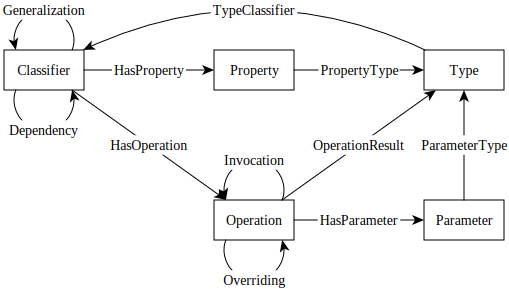
\includegraphics[width=0.8\textwidth]{inc/model-graph.pdf}
\caption{Граф модели объектно-ориентированной программы}
\label{fig:model-graph}
\end{figure}

\section{Алгоритм поиска шаблона в модели объектно-ориентированной программы}

Основная идея алгоритма в том, что нужно построить графы для модели программы
и шаблона и выполнить поиск изоморфных шаблону подграфов модели.
Определим необходимые функции и используемые алгоритмы.

\textbf{Определение}. $\textrm{INDIR\_GENERALS}: Classifier \to 2^{Classifier}$
--- множество всех ненапрямую базовых классов.

$\textrm{INDIR\_GENERALS}(c) = \begin{cases}
\varnothing \ \textrm{, если} \ c.generals = \varnothing \\
\{ x : (\exists g \in c.generals)(x \in \textrm{INDIR\_GENERALS}(g)) \}
\end{cases}
$

\textbf{Определение}. $\textrm{DOVERRID}: Operation \times 2^{Classifier} \to 2^{Operation}$
--- множество переопределяемых операций в заданных классах

$\textrm{DOVERRID}(op, classifiers) = \{ x : x = op \land (\exists g \in classifiers)(x \in g.operations) \}$

\textbf{Определение}. $\textrm{IOVERRID}: Operation \times 2^{Classifier} \to 2^{Operation}$
--- множество переопределяемых операций в заданных классах и их базовых классах

$\textrm{IOVERRID}(op, C) = \begin{cases}
\varnothing \ \textrm{, если} \ C = \varnothing \\
\textrm{DOVERRID}(op, C) \ \textrm{, если} \ \textrm{DOVERRID}(op, C) \ne \varnothing \\
\textrm{IOVERRID}(op, \{ s : (\exists c \in C)(s \in c.generals) \})
\end{cases}
$

\textbf{Определение}. $\textrm{OVERRIDDEN}: Operation \to 2^{Operation}$
--- множество переопределяемых операций

$\textrm{OVERRIDDEN}(operation) = \textrm{IOVERRID}(operation, operation.owner.generals)$

\textbf{Определение}. Алгоритм построения графа модели объектно-ориентированной программы.

\textbf{Входные данные}: $model$ --- модель программы;

\textbf{Результат}: $G$ --- граф модели программы.

\begin{algorithmic}
\Function{model\_graph}{$model$}
    \State $E \gets \varnothing$
    \ForAll{ $classifier \in model.classifiers$ }
        \ForAll{ $general \in$ \Call{indir\_generals}{$classifier$} }
            \State $E \gets E \cup \{ ( classifier, general, Generalization ) \}$
        \EndFor
        \ForAll{ $supplier \in classifier.suppliers$ }
            \State $E \gets E \cup \{ ( classifier, supplier, Dependency ) \}$
        \EndFor
        \ForAll{ $property \in classifier.properties$ }
            \State $E \gets E \cup \{ ( classifier, property, HasProperty ) \}$
            \State $E \gets E \cup \{ ( property, property.type, PropertyType ) \}$
            \State $E \gets E \cup \{ ( property.type, property.type.classifier, TypeClassifier ) \}$
        \EndFor
        \ForAll{ $operation \in classifier.operations$ }
            \State $E \gets E \cup \{ ( classifier, operation, HasOperation ) \}$
            \If{ $operation.result \ne \varnothing$ }
                \State $E \gets E \cup \{ ( classifier, operation.result, Dependency ) \}$
                \State $E \gets E \cup \{ ( operation, operation.result, OperationResult ) \}$
                \State $E \gets E \cup \{ ( operation.result, operation.result.classifier, TypeClassifier ) \}$
            \EndIf
            \ForAll{ $invoked \in operation.invocations$ }
                \State $E \gets E \cup \{ ( operation, invoked, Invocation ) \}$
            \EndFor
            \State $overidden \gets$ \Call{overridden}{$operation$}
            \If{ $overidden \ne \varnothing$ }
                \State $E \gets E \cup \{ ( operation, x, Overriding ) : \{ x \} \subseteq overridden \}$
            \EndIf
            \ForAll{ $parameter \in operation.parameters$ }
                \State $E \gets E \cup \{ ( classifier, parameter.type.classifier, Dependency ) \}$
                \State $E \gets E \cup \{ ( operation, parameter, HasParameters ) \}$
                \State $E \gets E \cup \{ ( parameter, parameter.type, ParameterType ) \}$
                \State $E \gets E \cup \{ ( parameter.type, parameter.type.classifier, TypeClassifier ) \}$
            \EndFor
        \EndFor
    \EndFor
    \State $V \gets \varnothing$
    \State $L \gets \varnothing$
    \ForAll{ $(u, v, l) \in E$ }
        \State $V \gets V \cup \{ u, v \}$
        \State $L \gets L \cup \{ l \}$
    \EndFor
    \State \Return $(V, L, E)$
\EndFunction
\end{algorithmic}

\textbf{Определение}. Алгоритм поиска шаблона в модели объектно-ориентированной программы.

\textbf{Входные данные}:
\begin{itemize}
\item $model_{target}$ --- модель программы;
\item $model_{pattern}$ --- модель шаблона.
\end{itemize}

\textbf{Результат}: $\{ \{ ( object_{target}, object_{pattern} ) \} \}$
--- множество вариантов соответствий объектов модели программы шаблону.

\begin{algorithmic}
\Function{match\_model}{$model_{target}$, $model_{pattern}$}
    \State $G_{target} \gets$ \Call{model\_graph}{$model_{target}$}
    \State $G_{pattern} \gets$ \Call{model\_graph}{$model_{pattern}$}
    \State \Return \Call{match\_graph}{component, $G_{pattern}$}
\EndFunction
\end{algorithmic}
